\documentclass{article}
\usepackage{enumitem}
\usepackage{outlines}
\usepackage{amsfonts}
\usepackage{amssymb}
\usepackage{amsmath}
\usepackage{wrapfig}
\usepackage{float}
\usepackage{xcolor}
\usepackage{titlesec}

\newcommand{\tri}[2] {#1^{\Delta #2}}

\usepackage{tikz,tikz-3dplot}
\usetikzlibrary{scopes}
\usepackage{verbatim}

\tdplotsetmaincoords{70}{40}
  
\setcounter{secnumdepth}{4}
\titleformat{\paragraph}
{\normalfont\normalsize\bfseries}{\theparagraph}{1em}{}
\titlespacing*{\paragraph}
{0pt}{3.25ex plus 1ex minus .2ex}{1.5ex plus .2ex}


\title{Some title containing the words ``triangular'', ``simplicial'', and ``numbers'', e.g. this one}
\date{\today}
\author{Andrew Gleeson}
\begin{document}
\maketitle

\begin{abstract}

Triangular numbers are positive integers with properties related to triangles. Graphically, they can be represented as the number of points in $\mathbb{Z}^{2}$ bounded by a right isoceles triangle.  They can also be viewed as $\sum_{i=1}^n i$, which is known to be  $\frac{n(n+1)}{2}$. Triangular numbers can be generalized to simplex numbers, which are analogous to triangular numbers in any dimension. Triangular numbers show up often across various areas of mathematics, mostly in combinatorics. Although some of the included results have been known for centuries, I independently arrived at many of the results before finding any previous work. This paper is intended to describe the results, many of which can be shown though very elegant proofs, and my journey to them.

\end{abstract}

\section{Introduction}

The concept of triangular numbers is intriguing. Most people are very
familiar with square numbers ($n^2$), but we don't put much thought
into why a square is chosen as the shape (Figure ~\ref{square}). Geometrically, there are
other very interesting \begin{wrapfigure}{r}{0.5\textwidth}

\centering
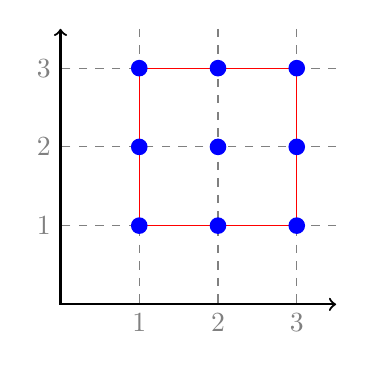
\begin{tikzpicture}
\foreach \x in {1,...,3}
     		\draw[dashed, gray] (\x,3.5) -- (\x,0)
			node[anchor=north] {\x};		
\foreach \y in {1,...,3}
     		\draw[dashed, gray] (3.5,\y) -- (0,\y)
			node[anchor=east] {\y};
\draw [<->, black, thick] (0,3.5) -- (0,0) -- (3.5,0);
\draw[red] (3,1) -- (3,3) -- (1,3) -- (1,1) -- cycle ;
\foreach \x in {1,...,3}
	\foreach \y in {1,...,3}
		\fill [blue] (\x, \y) circle [radius=3pt];
\end{tikzpicture}
\caption{$3^2 = 9$\label{square}}

\end{wrapfigure}
shapes. Two shapes that stand out are the
triangle, which has the least number of verticies required to bound an area in two-dimensional space, and the circle, which has an infinite
number of vertices. All other polygons are somewhere between the
two. So, it would seem that triangles, like squares, should be similarly important.
A square number can be thought of as the number of points is $\mathbb{Z}^2$ bounded by a square. They can also be viewed as $\sum_{i=1}^{n}n$ and $n^2$.

\begin{wrapfigure}{r}{0.5\textwidth}
\centering
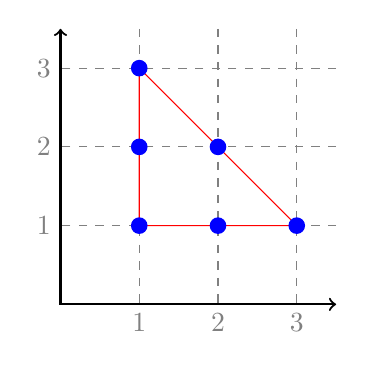
\begin{tikzpicture}
\foreach \x in {1,...,3}
     		\draw[dashed, gray] (\x,3.5) -- (\x,0)
			node[anchor=north] {\x};			
\foreach \y in {1,...,3}
     		\draw[dashed, gray] (3.5,\y) -- (0,\y)
			node[anchor=east] {\y};
\draw [<->, black, thick] (0,3.5) -- (0,0) -- (3.5,0);
\draw[red] (3,1) -- (1,3) -- (1,1) -- cycle ;
\fill [blue] (3, 1) circle [radius=3pt];
\fill [blue] (2, 1) circle [radius=3pt];
\fill [blue] (1, 1) circle [radius=3pt];
\fill [blue] (1, 2) circle [radius=3pt];
\fill [blue] (1, 3) circle [radius=3pt];
\fill [blue] (2, 2) circle [radius=3pt];
\end{tikzpicture}
\caption{$T_3 = 6$\label{triangular}}
%\vspace{-10pt}
\end{wrapfigure}
\section{Triangular Numbers}
To form a triangular number, we can instead bound the points with a right isoceles triangle. (Figure ~\ref{triangular})
What would a triangular number be?
If we examine the triangular numbers, we can see that in each successive row, the number of dots increments by one. So, we can express the $n$th triangular number $T_n$ as the sum of the numbers 1 to $n$.\\
\\
$T_n = 1+2+...+n = \sum_{i = 1}^n i = \frac{n(n+1)}{2}$\\

With some simple steps, we can transform triangular numbers into something much more well known.

\begin{align*}
T_n &= \frac{n(n+1)}{2} \\
&= \frac{(n+1)!}{2! (n-1)!}\quad\text{(rewrite using factorials)}\\
&= \frac{k!}{2! (k-2)!} \quad\text{(let k = n+1)}\\
&= \binom{k}{2} \quad\text{(by the definition of a binomial coefficient)}\\
&= \binom{n+1}{2} \quad\text{(substitute)}
\end{align*}

In plain English, this means that the $n$th triangular number is the number of combinations of 2 items from a set of n+1 items. This fact connects us to the world of combinatorics. However, I decided to not delve into combinatorics to find properties of triangular numbers. It is possible to manipulate already-known properties of binomial coefficients to say something about triangular numbers, but that would mean deviating from the beautiful geometry of triangular numbers. There exist many other properties of triangular numbers that have elegant geometric proofs, which was the path of interest to me.\\

For example, two important triangular identities are $T_n + T_{n-1} = n^2$ and $T_n - T_{n-1} = n$. These identities are essential to the relationship between triangular numbers and exponentiation. It means that any square number, or any integer, can by represented as the sum or difference of two triangular numbers.

\begin{figure}[H]
\centering

\begin{centering}

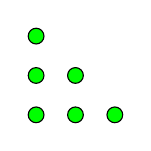
\begin{tikzpicture}[scale=0.5]
	\draw[fill=green] (0,0) circle [radius=0.2cm];
	\draw[fill=green] (0,1) circle [radius=0.2cm];
	\draw[fill=green] (0,2) circle [radius=0.2cm];
	\draw[fill=green] (1,0) circle [radius=0.2cm];
	\draw[fill=green] (1,1) circle [radius=0.2cm];
	\draw[fill=green] (2,0) circle [radius=0.2cm];
\end{tikzpicture}
\quad
\huge{+}
\quad
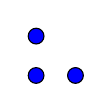
\begin{tikzpicture}[scale=0.5]
	\draw[fill=blue] (0,0) circle [radius=0.2cm];
	\draw[fill=blue] (1,0) circle [radius=0.2cm];
	\draw[fill=blue] (0,1) circle [radius=0.2cm];
\end{tikzpicture}
\quad
\huge{=}
\quad
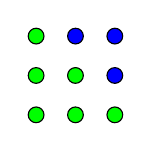
\begin{tikzpicture}[scale=0.5]
	\draw[fill=green] (0,0) circle [radius=0.2cm];
	\draw[fill=green] (0,1) circle [radius=0.2cm];
	\draw[fill=green] (0,2) circle [radius=0.2cm];
	\draw[fill=green] (1,0) circle [radius=0.2cm];
	\draw[fill=green] (1,1) circle [radius=0.2cm];
	\draw[fill=green] (2,0) circle [radius=0.2cm];
	
	\draw[fill=blue] (2,2) circle [radius=0.2cm];
	\draw[fill=blue] (2,1) circle [radius=0.2cm];
	\draw[fill=blue] (1,2) circle [radius=0.2cm];
\end{tikzpicture}
\end{centering}
\caption{$T_3 + T_2 = 3^2$\label{tnplustnminus1l}}
\end{figure}
\begin{figure}[H]
\centering
\include{tnminustnminus1}
\caption{$T_3 - T_2 = 3$\label{tnminustnminus1l}}
\end{figure}


\subsection{Properties}

Many properties of triangular numbers can be shown geometrically, while others are shown through the manipulation of equations.

For example, the identity $T_{2n} = 3\cdot T_n + T_{n-1}$ can be shown through a simple graphic.
\begin{figure}[H]
\centering

\begin{centering}

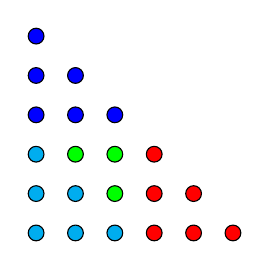
\begin{tikzpicture}
	\draw[fill=cyan] (0,0) circle [radius=0.1cm];
	\draw[fill=cyan] (0,0.5) circle [radius=0.1cm];
	\draw[fill=cyan] (0,1) circle [radius=0.1cm];
	\draw[fill=blue] (0,1.5) circle [radius=0.1cm];
	\draw[fill=blue] (0,2) circle [radius=0.1cm];
	\draw[fill=blue] (0,2.5) circle [radius=0.1cm];
	
	\draw[fill=cyan] (0.5,0) circle [radius=0.1cm];
	\draw[fill=cyan] (0.5,0.5) circle [radius=0.1cm];
	\draw[fill=green] (0.5,1) circle [radius=0.1cm];
	\draw[fill=blue] (0.5,1.5) circle [radius=0.1cm];
	\draw[fill=blue] (0.5,2) circle [radius=0.1cm];
	
	\draw[fill=cyan] (1,0) circle [radius=0.1cm];
	\draw[fill=green] (1,0.5) circle [radius=0.1cm];
	\draw[fill=green] (1,1) circle [radius=0.1cm];
	\draw[fill=blue] (1,1.5) circle [radius=0.1cm];
	
	\draw[fill=red] (1.5,0) circle [radius=0.1cm];
	\draw[fill=red] (1.5,0.5) circle [radius=0.1cm];
	\draw[fill=red] (1.5,1) circle [radius=0.1cm];
	
	\draw[fill=red] (2,0) circle [radius=0.1cm];
	\draw[fill=red] (2,0.5) circle [radius=0.1cm];
	
	\draw[fill=red] (2.5,0) circle [radius=0.1cm];
\end{tikzpicture}
\quad
\huge{$= 3\enspace\cdot$}
\enspace
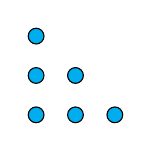
\begin{tikzpicture}
	\draw[fill=cyan] (0,0) circle [radius=0.1cm];
	\draw[fill=cyan] (0,0.5) circle [radius=0.1cm];
	\draw[fill=cyan] (0,1) circle [radius=0.1cm];
	
	\draw[fill=cyan] (0.5,0) circle [radius=0.1cm];
	\draw[fill=cyan] (0.5,0.5) circle [radius=0.1cm];
	
	\draw[fill=cyan] (1,0) circle [radius=0.1cm];
\end{tikzpicture}
\quad
\huge{+}
\quad
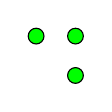
\begin{tikzpicture}

	\draw[fill=green] (0.5,1) circle [radius=0.1cm];
	
	\draw[fill=green] (1,0.5) circle [radius=0.1cm];
	\draw[fill=green] (1,1) circle [radius=0.1cm];
\end{tikzpicture}
\end{centering}
\caption{$T_{6} = 3 \cdot T_3 + T_2$\label{T2n}}
\end{figure}

However, some identities  lend themselves to an algebraic derivation.

\begin{enumerate}
  \item $(T_n)^2 = \sum_{i=1}^n i^3$
  \item $T_{a+b} = T_a + T_b + 2ab$
  \item $T_{ab} = T_a T_b + T_{a-1}T_{b-1}$
  \item $T_n - T_{n-k} = \frac{k}{2} (2n + 1 - k)$
\end{enumerate}

And , by using (4), it can be shown that the difference of two triangular numbers will never be a perfect square if $k$ is two or greater.\\

Some other identities are even more obscure. Gauss, with his Eureka Theorem, showed that any integer is the sum of at most three triangular numbers. All even perfect numbers (a number which equals the sum of its proper divisors excluding itself) are triangular numbers.

\subsubsection{Reciprocal Infinite Series}

There is a nice cleanliness to the reciprocal sum of all triangular numbers. By a simple telescopic series, $\sum_{n=1}^{\infty} \frac{1}{T_n} = 2$.

Some mathematicians have generalized this to cover $T_{mn+r}$ instead of just $T_n$. They found that
\begin{multline*}
		\sum_{n=0}^\infty \frac{1}{T_{mn+r}} = 
		\frac{2}{m} \sum\limits_{0<j<m/2} \left\{ 
		\left[
			\cos \left(\frac{2 \pi j (r+1)}{m} \right) - \cos \left( \frac{2 \pi j r}{m} \right)
		\right] \right. \\
		\left. \cdot \ln \left[ 
		2 - \cos \left( \frac{2 \pi j}{m} \right)
		\right]
		- \left[ \sin \left(\frac{2 \pi j (r+1)}{m} \right) - \sin \left( \frac{2 \pi j r}{m} \right) \right] \right. \\
		\left. \cdot \frac{\pi (m - 2j)}{m}
		\right\} + 2 \delta_{mr} + \varepsilon_m \cdot (-1)^{r+1} 2 \ln(2)
\end{multline*}

Note: $\delta_{ij}$ is the Kronecker delta function, which is 0 when $i=j$ and 1 otherwise. $\varepsilon_i$ returns 1 if $i$ is even, and 0 if $i$ is odd.\\

Plugging in specific $m$ and $r$:

\begin{itemize}
	\item $\sum_{n=0}^\infty \frac{1}{T_{2n+2}} = 2 - 2 \ln 2$
	\item $\sum_{n=0}^\infty \frac{1}{T_{3n+1}} = \frac{2 \pi \sqrt{3}}{9}$
	\item $\sum_{n=0}^\infty \frac{1}{T_{4n+1}} = \frac{\pi}{4} + \frac{3}{2}\ln 2$
	\item $\sum_{n=0}^\infty \frac{1}{T_{4n+2}} = \frac{\pi}{4} - \frac{3}{2}\ln 2$
	\item $\sum_{n=0}^\infty \frac{1}{T_{4n+3}} = - \frac{\pi}{4} + \frac{5}{2}\ln 2$
\end{itemize}

\paragraph{Example  - $T_{2n+2}$}

\begin{align*}
\sum_{n=0}^\infty \frac{1}{T_{2n+2}} = 
		\frac{2}{2} \sum\limits_{0<j<2/2} \left\{ 
		\left[
			\cos \left(\frac{2 \pi j (2+1)}{2} \right) - \cos \left( \frac{2 \pi j (2)}{2} \right)
		\right] \right. \\
		\left. \cdot \ln \left[ 
		2 - \cos \left( \frac{2 \pi j}{2} \right)
		\right]
		- \left[ \sin \left(\frac{2 \pi j (2+1)}{2} \right) - \sin \left( \frac{2 \pi j (2)}{2} \right) \right] \right. \\
		\left. \cdot \frac{\pi (2 - 2j)}{2}
		\right\} + 2 \delta_{2,2} + \varepsilon_2 \cdot (-1)^{2+1} 2 \ln(2)\\
		\\
		= 2 \delta_{2,2}-\varepsilon_{2} \cdot 2 \ln 2\\
		= 2 \cdot 1 - 1\cdot 2 \ln 2\\
		= 2 - 2 \ln 2
\end{align*}

\paragraph{Example  - $T_{3n+1}$}

\begin{align*}
		\sum_{n=0}^\infty \frac{1}{T_{3n+1}} = 
		\frac{2}{3} \sum\limits_{0<j<3/2} \left\{ 
		\left[
			\cos \left(\frac{2 \pi j (1+1)}{3} \right) - \cos \left( \frac{2 \pi j (1)}{3} \right)
		\right] \right. \\
		\left. \cdot \ln \left[ 
		2 - \cos \left( \frac{2 \pi j}{3} \right)
		\right]
		- \left[ \sin \left(\frac{2 \pi j (1+1)}{3} \right) - \sin \left( \frac{2 \pi j (1)}{3} \right) \right] \right. \\
		\left. \cdot \frac{\pi (3 - 2j)}{3}
		\right\} + 2 \delta_{3,1} + \varepsilon_3 \cdot (-1)^{1+1} 2 \ln(2)\\
		\\
		= \frac{2}{3} \left\{ 0 - [-\sqrt{3}] \cdot \frac{\pi}{3} \right\} + 2 \cdot 0 + 0 \cdot 2 \ln 2\\
		= \frac{2 \pi \sqrt{3} }{9}
\end{align*}

At the very least, it is remarkable that there are several similar terms in the results.

\begin{wrapfigure}{R}{3cm}
\documentclass{article}
\usepackage{tikz,tikz-3dplot}
\usetikzlibrary{scopes}
\usepackage{verbatim}

\tdplotsetmaincoords{70}{40}

\begin{document}
\begin{centering}

\def\s{2.5} % F_g

\begin{tikzpicture}[>=stealth,tdplot_main_coords]
    	\coordinate (O) at (0,0,0);
   	\coordinate (A) at (0,\s,0);
   	\coordinate (B) at ({sqrt(3)/2*\s},{\s/2},0);
	\coordinate (C) at ({sqrt(3)/6*\s},{\s/2},{sqrt(6)/3*\s});
    
    	%\draw[->] (O) -- (6,0,0);
    	%\draw[->] (O) -- (0,6,0);
    	%\draw[->] (O) -- (0,0,6);
    
    	
    	\draw[blue,fill=yellow!50] (O) -- (A) -- (B) -- cycle;
    	\draw[blue,fill=red!20] (O) -- (A) -- (C) -- cycle;
    	
    	\draw[blue,fill=green!10] (A) -- (B) -- (C) -- cycle;
    	
    	\draw[fill=red]  ($(A)!0.5!(B) $)  circle [radius=0.075cm];
    	\draw[fill=blue]  ($(A)!0.5!(C) $)  circle [radius=0.075cm];
    	\draw[fill=red]  ($(O)!0.5!(A) $)  circle [radius=0.075cm];
    	
    	\draw[fill=red] (A) circle [radius=0.1cm];
    	\draw[blue,fill=blue!10,opacity=0.6] (O) -- (B) -- (C) -- cycle;

	\draw[fill=red] (O) circle [radius=0.1cm];
    	
    	\draw[fill=red] (B) circle [radius=0.1cm];
    	\draw[fill=green] (C) circle [radius=0.1cm];
    	
    	
    	\draw[fill=red]  ($(O)!0.5!(B) $)  circle [radius=0.075cm];
    	\draw[fill=blue]  ($(O)!0.5!(C) $)  circle [radius=0.075cm];
    	
    	\draw[red, thick] (O) -- (B) -- (A) -- cycle;
    	\draw[blue, thick] ($(A)!0.5!(C) $) -- ($(C)!0.5!(B) $) --($(C)!0.5!(O) $) -- cycle;
    	
    	
    	
    	\draw[fill=blue]  ($(C)!0.5!(B) $)  circle [radius=0.075cm];
    	
    	%\foreach \xy in {O, A, B, C}{
	%	\node at (\xy) {\xy};
	%}
\end{tikzpicture}


\huge{$\Downarrow$}\\

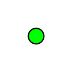
\begin{tikzpicture}
	\draw[fill=green] (0,0) circle [radius=0.1cm];
\end{tikzpicture}\\
\huge{+}\\
\vspace{0.3cm}
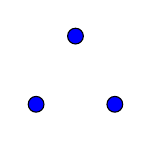
\begin{tikzpicture}
	\draw[fill=blue] (0,0) circle [radius=0.1cm];
	\draw[fill=blue] (1,0) circle [radius=0.1cm];
	\draw[fill=blue] ({1/2},{sqrt(3)/2}) circle [radius=0.1cm];
\end{tikzpicture}\\
\huge{+}\\
\vspace{0.3cm}
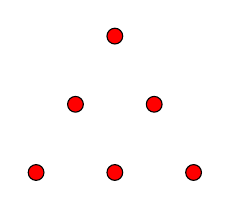
\begin{tikzpicture}
	\draw[fill=red] (0,0) circle [radius=0.1cm];
	\draw[fill=red] (1,0) circle [radius=0.1cm];
	\draw[fill=red] ({1/2},{sqrt(3)/2}) circle [radius=0.1cm];
	\draw[fill=red] ({-1/2},{-sqrt(3)/2}) circle [radius=0.1cm];
	\draw[fill=red] ({1/2},{-sqrt(3)/2}) circle [radius=0.1cm];
	\draw[fill=red] ({3/2},{-sqrt(3)/2}) circle [radius=0.1cm];
\end{tikzpicture}\\
\end{centering}
\end{document}
\caption{$\tri{3}{3}= 10$\label{tetrahedral}}
\end{wrapfigure}
\section{Simplex Numbers}

Triangular numbers can be generalized to any dimension by turning them into simplexes. A simplex is a generalization of the idea of a triangle or tetrahedron to any dimension. For example, a triangle is a 2-simplex, meaning a simplex in two dimensions. A tetrahedron is a 3-simplex - and the list goes on. I will use the notation $\tri{n}{d}$ to signify the $n$th $d$-simplex number.

\subsection{Tetrahedral Numbers}
We have cube numbers, ($n^3$ or $\sum_{i=1}^{n}n^2$) --- what would tetrahedral numbers be? (Figure ~\ref{tetrahedral}) In the same way that a cube is made up of squares, a tetrahedral number is the sum of triangular numbers.

$\tri{n}{3} = \tri{1}{2}+\tri{2}{2}+...+\tri{n}{2} = \sum_{i=1}^n \tri{i}{2} = \frac{n(n+1)(n+2)}{6}$

\subsection{Fourth dimension and beyond}
Many of the properties of triangular and tetrahedral numbers hold true for any arbitrary dimension. We saw that $\tri{n}{2}$ is the sum from 1 to n, and that $\tri{n}{3}$ was the sum of the first $n$ triangular numbers. This carries over:
\begin{align*}
\tri{n}{d} &= \sum_{i=1}^n \tri{i}{d-1}
\end{align*}
The combinatoric identity also generalizes:
\begin{align*}
 \tri{n}{d} = \binom{n+d-1}{d}
 \end{align*}
 
 The reciprocal infinite sum generalizes wonderfully, giving us
 \begin{align*}
 \sum_{n=1}^{\infty} \frac{1}{\tri{n}{d}} = \frac{d}{d-1}
  \end{align*}
 However, some properties do not translate easily. The square identity, $n^2 = T_n + T_{n-1}$, is very simple. Unfortunately, it is significantly more complex for cubes:
 
 \begin{align*}
 n^3 = \tri{n}{3} + \tri{(2n-2)}{3} - 3 \tri{(n-2)}{3}
 \end{align*}
 
 This can be shown by visualizing tetrahedral numbers as the sum of triangular numbers, and cubes as the sums of square numbers.\\

\begin{figure}[H]
\centering

\begin{centering}

\huge{$\color{cyan}n^3\color{black}=$}
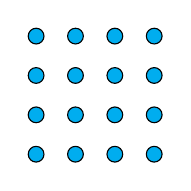
\begin{tikzpicture}
	\draw[fill=cyan] (0,0) circle [radius=0.1cm];
	\draw[fill=cyan] (0,0.5) circle [radius=0.1cm];
	\draw[fill=cyan] (0,1) circle [radius=0.1cm];
	\draw[fill=cyan] (0,1.5) circle [radius=0.1cm];
	
	\draw[fill=cyan] (0.5,0) circle [radius=0.1cm];
	\draw[fill=cyan] (0.5,0.5) circle [radius=0.1cm];
	\draw[fill=cyan] (0.5,1) circle [radius=0.1cm];
	\draw[fill=cyan] (0.5,1.5) circle [radius=0.1cm];
	
	\draw[fill=cyan] (1,0) circle [radius=0.1cm];
	\draw[fill=cyan] (1,0.5) circle [radius=0.1cm];
	\draw[fill=cyan] (1,1) circle [radius=0.1cm];
	\draw[fill=cyan] (1,1.5) circle [radius=0.1cm];
	
	\draw[fill=cyan] (1.5,0) circle [radius=0.1cm];
	\draw[fill=cyan] (1.5,0.5) circle [radius=0.1cm];
	\draw[fill=cyan] (1.5,1) circle [radius=0.1cm];
	\draw[fill=cyan] (1.5,1.5) circle [radius=0.1cm];
\end{tikzpicture}
\quad
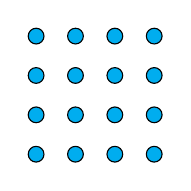
\begin{tikzpicture}
	\draw[fill=cyan] (0,0) circle [radius=0.1cm];
	\draw[fill=cyan] (0,0.5) circle [radius=0.1cm];
	\draw[fill=cyan] (0,1) circle [radius=0.1cm];
	\draw[fill=cyan] (0,1.5) circle [radius=0.1cm];
	
	\draw[fill=cyan] (0.5,0) circle [radius=0.1cm];
	\draw[fill=cyan] (0.5,0.5) circle [radius=0.1cm];
	\draw[fill=cyan] (0.5,1) circle [radius=0.1cm];
	\draw[fill=cyan] (0.5,1.5) circle [radius=0.1cm];
	
	\draw[fill=cyan] (1,0) circle [radius=0.1cm];
	\draw[fill=cyan] (1,0.5) circle [radius=0.1cm];
	\draw[fill=cyan] (1,1) circle [radius=0.1cm];
	\draw[fill=cyan] (1,1.5) circle [radius=0.1cm];
	
	\draw[fill=cyan] (1.5,0) circle [radius=0.1cm];
	\draw[fill=cyan] (1.5,0.5) circle [radius=0.1cm];
	\draw[fill=cyan] (1.5,1) circle [radius=0.1cm];
	\draw[fill=cyan] (1.5,1.5) circle [radius=0.1cm];
\end{tikzpicture}
\quad
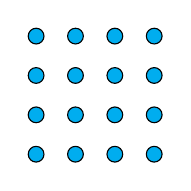
\begin{tikzpicture}
	\draw[fill=cyan] (0,0) circle [radius=0.1cm];
	\draw[fill=cyan] (0,0.5) circle [radius=0.1cm];
	\draw[fill=cyan] (0,1) circle [radius=0.1cm];
	\draw[fill=cyan] (0,1.5) circle [radius=0.1cm];
	
	\draw[fill=cyan] (0.5,0) circle [radius=0.1cm];
	\draw[fill=cyan] (0.5,0.5) circle [radius=0.1cm];
	\draw[fill=cyan] (0.5,1) circle [radius=0.1cm];
	\draw[fill=cyan] (0.5,1.5) circle [radius=0.1cm];
	
	\draw[fill=cyan] (1,0) circle [radius=0.1cm];
	\draw[fill=cyan] (1,0.5) circle [radius=0.1cm];
	\draw[fill=cyan] (1,1) circle [radius=0.1cm];
	\draw[fill=cyan] (1,1.5) circle [radius=0.1cm];
	
	\draw[fill=cyan] (1.5,0) circle [radius=0.1cm];
	\draw[fill=cyan] (1.5,0.5) circle [radius=0.1cm];
	\draw[fill=cyan] (1.5,1) circle [radius=0.1cm];
	\draw[fill=cyan] (1.5,1.5) circle [radius=0.1cm];
\end{tikzpicture}

\vspace{12pt}
\huge{$= \color{red}\tri{n}{3} \color{black}+ \color{green}? \color{black}= $}
\enspace
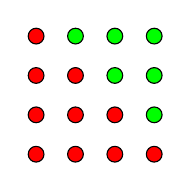
\begin{tikzpicture}
	\draw[fill=red] (0,0) circle [radius=0.1cm];
	\draw[fill=red] (0,0.5) circle [radius=0.1cm];
	\draw[fill=red] (0,1) circle [radius=0.1cm];
	\draw[fill=red] (0,1.5) circle [radius=0.1cm];
	
	\draw[fill=red] (0.5,0) circle [radius=0.1cm];
	\draw[fill=red] (0.5,0.5) circle [radius=0.1cm];
	\draw[fill=red] (0.5,1) circle [radius=0.1cm];
	\draw[fill=green] (0.5,1.5) circle [radius=0.1cm];
	
	\draw[fill=red] (1,0) circle [radius=0.1cm];
	\draw[fill=red] (1,0.5) circle [radius=0.1cm];
	\draw[fill=green] (1,1) circle [radius=0.1cm];
	\draw[fill=green] (1,1.5) circle [radius=0.1cm];
	
	\draw[fill=red] (1.5,0) circle [radius=0.1cm];
	\draw[fill=green] (1.5,0.5) circle [radius=0.1cm];
	\draw[fill=green] (1.5,1) circle [radius=0.1cm];
	\draw[fill=green] (1.5,1.5) circle [radius=0.1cm];
\end{tikzpicture}
\quad
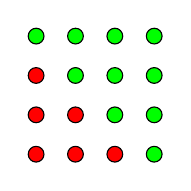
\begin{tikzpicture}

	\draw[fill=red] (0,0) circle [radius=0.1cm];
	\draw[fill=red] (0,0.5) circle [radius=0.1cm];
	\draw[fill=red] (0,1) circle [radius=0.1cm];
	\draw[fill=green] (0,1.5) circle [radius=0.1cm];
	
	\draw[fill=red] (0.5,0) circle [radius=0.1cm];
	\draw[fill=red] (0.5,0.5) circle [radius=0.1cm];
	\draw[fill=green] (0.5,1) circle [radius=0.1cm];
	\draw[fill=green] (0.5,1.5) circle [radius=0.1cm];
	
	\draw[fill=red] (1,0) circle [radius=0.1cm];
	\draw[fill=green] (1,0.5) circle [radius=0.1cm];
	\draw[fill=green] (1,1) circle [radius=0.1cm];
	\draw[fill=green] (1,1.5) circle [radius=0.1cm];
	
	\draw[fill=green] (1.5,0) circle [radius=0.1cm];
	\draw[fill=green] (1.5,0.5) circle [radius=0.1cm];
	\draw[fill=green] (1.5,1) circle [radius=0.1cm];
	\draw[fill=green] (1.5,1.5) circle [radius=0.1cm];
\end{tikzpicture}
\quad
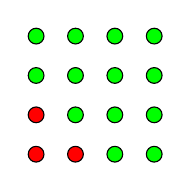
\begin{tikzpicture}
	\draw[fill=red] (0,0) circle [radius=0.1cm];
	\draw[fill=red] (0,0.5) circle [radius=0.1cm];
	\draw[fill=green] (0,1) circle [radius=0.1cm];
	\draw[fill=green] (0,1.5) circle [radius=0.1cm];
	
	\draw[fill=red] (0.5,0) circle [radius=0.1cm];
	\draw[fill=green] (0.5,0.5) circle [radius=0.1cm];
	\draw[fill=green] (0.5,1) circle [radius=0.1cm];
	\draw[fill=green] (0.5,1.5) circle [radius=0.1cm];
	
	\draw[fill=green] (1,0) circle [radius=0.1cm];
	\draw[fill=green] (1,0.5) circle [radius=0.1cm];
	\draw[fill=green] (1,1) circle [radius=0.1cm];
	\draw[fill=green] (1,1.5) circle [radius=0.1cm];
	
	\draw[fill=green] (1.5,0) circle [radius=0.1cm];
	\draw[fill=green] (1.5,0.5) circle [radius=0.1cm];
	\draw[fill=green] (1.5,1) circle [radius=0.1cm];
	\draw[fill=green] (1.5,1.5) circle [radius=0.1cm];
\end{tikzpicture}

\vspace{12pt}
\large{fill out \color{green}tetrahedral}
\quad
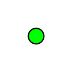
\begin{tikzpicture}
	\draw[fill=green] (1,1) circle [radius=0.1cm];
\end{tikzpicture}
\quad
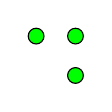
\begin{tikzpicture}
	\draw[fill=green] (0.5,0.5) circle [radius=0.1cm];
	\draw[fill=green] (0,0.5) circle [radius=0.1cm];
	\draw[fill=green] (0.5,0) circle [radius=0.1cm];
\end{tikzpicture}
\quad
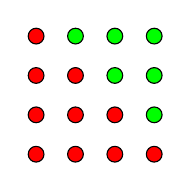
\begin{tikzpicture}
	\draw[fill=red] (0,0) circle [radius=0.1cm];
	\draw[fill=red] (0,0.5) circle [radius=0.1cm];
	\draw[fill=red] (0,1) circle [radius=0.1cm];
	\draw[fill=red] (0,1.5) circle [radius=0.1cm];
	
	\draw[fill=red] (0.5,0) circle [radius=0.1cm];
	\draw[fill=red] (0.5,0.5) circle [radius=0.1cm];
	\draw[fill=red] (0.5,1) circle [radius=0.1cm];
	\draw[fill=green] (0.5,1.5) circle [radius=0.1cm];
	
	\draw[fill=red] (1,0) circle [radius=0.1cm];
	\draw[fill=red] (1,0.5) circle [radius=0.1cm];
	\draw[fill=green] (1,1) circle [radius=0.1cm];
	\draw[fill=green] (1,1.5) circle [radius=0.1cm];
	
	\draw[fill=red] (1.5,0) circle [radius=0.1cm];
	\draw[fill=green] (1.5,0.5) circle [radius=0.1cm];
	\draw[fill=green] (1.5,1) circle [radius=0.1cm];
	\draw[fill=green] (1.5,1.5) circle [radius=0.1cm];
\end{tikzpicture}
\quad
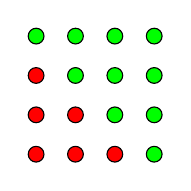
\begin{tikzpicture}

	\draw[fill=red] (0,0) circle [radius=0.1cm];
	\draw[fill=red] (0,0.5) circle [radius=0.1cm];
	\draw[fill=red] (0,1) circle [radius=0.1cm];
	\draw[fill=green] (0,1.5) circle [radius=0.1cm];
	
	\draw[fill=red] (0.5,0) circle [radius=0.1cm];
	\draw[fill=red] (0.5,0.5) circle [radius=0.1cm];
	\draw[fill=green] (0.5,1) circle [radius=0.1cm];
	\draw[fill=green] (0.5,1.5) circle [radius=0.1cm];
	
	\draw[fill=red] (1,0) circle [radius=0.1cm];
	\draw[fill=green] (1,0.5) circle [radius=0.1cm];
	\draw[fill=green] (1,1) circle [radius=0.1cm];
	\draw[fill=green] (1,1.5) circle [radius=0.1cm];
	
	\draw[fill=green] (1.5,0) circle [radius=0.1cm];
	\draw[fill=green] (1.5,0.5) circle [radius=0.1cm];
	\draw[fill=green] (1.5,1) circle [radius=0.1cm];
	\draw[fill=green] (1.5,1.5) circle [radius=0.1cm];
\end{tikzpicture}
\quad
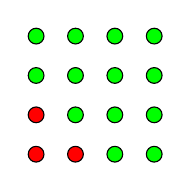
\begin{tikzpicture}
	\draw[fill=red] (0,0) circle [radius=0.1cm];
	\draw[fill=red] (0,0.5) circle [radius=0.1cm];
	\draw[fill=green] (0,1) circle [radius=0.1cm];
	\draw[fill=green] (0,1.5) circle [radius=0.1cm];
	
	\draw[fill=red] (0.5,0) circle [radius=0.1cm];
	\draw[fill=green] (0.5,0.5) circle [radius=0.1cm];
	\draw[fill=green] (0.5,1) circle [radius=0.1cm];
	\draw[fill=green] (0.5,1.5) circle [radius=0.1cm];
	
	\draw[fill=green] (1,0) circle [radius=0.1cm];
	\draw[fill=green] (1,0.5) circle [radius=0.1cm];
	\draw[fill=green] (1,1) circle [radius=0.1cm];
	\draw[fill=green] (1,1.5) circle [radius=0.1cm];
	
	\draw[fill=green] (1.5,0) circle [radius=0.1cm];
	\draw[fill=green] (1.5,0.5) circle [radius=0.1cm];
	\draw[fill=green] (1.5,1) circle [radius=0.1cm];
	\draw[fill=green] (1.5,1.5) circle [radius=0.1cm];
\end{tikzpicture}
\end{centering}
\caption{Cubes as a combination of tetrahedrals. Note: this is broken at the moment, will fix later}
\end{figure}
 
 \subsubsection*{Symbolic Proof}
 
 \begin{align*}
 n^3 &= \tri{n}{3} + \tri{(2n-2)}{3} - 3 \tri{(n-2)}{3}\\
 n^3 &= \frac{(n)(n+1)(n+2)}{6} + \frac{(2n-2)(2n-1)(2n)}{6} - \frac{3(n-2)(n-1)(n)}{6}\\
n^3 &= \frac{n^3 + 3n^2 + 2n}{6} + \frac{ 8n^3 - 12n^2 + 4n}{6} - \frac{3n^3 - 9n^2 + 6n}{6}\\
 n^3 &= \frac{n^3 + 3n^2 + 2n + 8n^3 - 12n^2 + 4n - 3n^3 + 9n^2 - 6n}{6}\\
 n^3 &= \frac{6n^3}{6} = n^3
 \end{align*}
 
 \section{Conclusion}

Hopefully, you agree that triangular and simplex numbers are interesting. Although the concept of a triangular number is exceedingly simple, they have a surprisingly broad scope and a powerful geometric appeal. Many of the results have a certain symmetry that falls from the underlying simplicity of the concept. Additionally, and more informally, following the triangular trail was a great deal of fun. Because triangular and simplicial numbers are relatively obscure, I was only able to find citations for many results after I knew exactly what I was looking for -- that is, I independantly derived them. For me, this fulfills the criteria for mathematical beauty.

\end{document}